%Aqui voce mostra que a heurística em si funciona (isto é, tem resultados parecidos com o do Emma). Eu acho que
%primeiro eu mostraria a heurística em si pra mostrar que o resultado perfeito (e inalcançável) é satisfatório quando
%comparado ao Emma (porque se não fosse, nem a melhor implementação teria resultado satisfatório). Em seguida, eu mostraria 
%a tua implementação. Depois, eu tentaria mostrar o quão 
%perto ou longe está o cálculo do numerador da heurística (link unit test - production method) na tua implementação vs o aspecto (Listing 5). 
%Bastaria mostrar precision e recall pra cada projeto. Lógico que, por conta de polimorfismo, etc, a implementação nunca será perfeita. 
%Mas saber o quão perto ou o quão longe está, seria interessante. Esse no fundo é o desafio principal por detrás do calculo da cobertura.
%Feito isso, aí sim eu rodaria nos 3 projetos e mostraria os resultados. Em resumo você começa num nível mais abstrato e termina na tua implementação
%(que revela o melhor que a gente consegue fazer na prática por enquanto)

\documentclass{sig-alternate}
\usepackage[utf8]{inputenc}
\usepackage{listings}
\usepackage{graphicx}
\usepackage{lipsum}
\usepackage{caption}
\usepackage{subcaption}
\usepackage{flushend}

\lstset{
language=Java,
basicstyle=\footnotesize,
showtabs=false, 
showspaces=false,
showstringspaces=false,
frame=single,
breaklines=true,
tabsize=2,
captionpos=b
}

\begin{document}

\conferenceinfo{MSR}{Mining Software Repositories '14}

\title{Calcuting Code Coverage Without Running the Tests:\\
A Heuristic Based on Static Code Analysis}

\numberofauthors{1}
\author{
\alignauthor
Mauricio F. Aniche, Gustavo A. Oliva, Marco A. Gerosa\\
\affaddr{Institute of Mathematics and Statistics}\\
\affaddr{University of São Paulo}\\
\email{\{aniche, goliva, gerosa\}@ime.usp.br}
}

\maketitle
\begin{abstract}

Code coverage is an important metric for software evolution and maintenance.
However, computing it requires building the project and executing its test suite.
This is unfeasible for large-scale mining software repositories studies. To this end,
we conceived and implemented a heuristic to calculate code coverage based on 
code static analysis. In this paper, we describe the heuristic, its implementation, 
and a preliminary evaluation on three industry projects. We evaluated our implementation by 
comparing its results to those produced by the popular code coverage tool Emma. Results showed that, 
although our implementation is not complete yet, its results were at least regular for two of the projects. 
These promising results showed that it might be suitable to use our implementation for mining studies.


\end{abstract}

%%%%%%%%%%%%%%%%%%%%%%%%%%%%%%%%%%%%%%%%%%%%%%%%%%%%%%%%%%%%%%%%%%%%%%%%%%%%%%%%%%%%%%%%%%
\section{Introduction}
\label{sec:intro}

One advantage of studies that make use of mining software repository techniques
is that they can leverage a large quantity of projects and data. This huge
amount of information allows researchers to validate hypotheses with more property.

Researchers can extract data from many different sources, 
such as source code repositories (a.k.a. version control systems), 
issue trackers, mailing lists, and so on. Most of these repositories 
store textual information, which is often easy to extract but hard to process. 
In the case of source code mining, a particular problem arises: some metrics 
require the code to be compiled first. And compiling code is a complicated task. 
Each project has its own build process and required libraries. Furthermore, 
it is common that many of these libraries are not available by the time 
researchers obtain the source code. Therefore, compiling and executing 
unit tests may not be feasible when conducting mining studies involving a large
quantity of projects.

An example of code metric that usually requires compiled code is \textit{code coverage}. 
This metric defines the percentage of production code that is covered 
by the test suite. To enable the calculation of code coverage for mining software
repository studies, we conceived a heuristic that does not require compiled code
and neither requires the test suite to be run. In this paper, we describe this heuristic,
its implementation, and its evaluation on three industry projects. 
We found out that, although our tool implementation is not fully completed yet, the 
proposed heuristic on how to calculate code coverage using static analysis seems valid. 

This paper is structured as follows. In Section \ref{sec-code-coverage}, 
we introduce the concept of code coverage. In Section \ref{sec-heuristic}, 
we present our heuristic. In Section \ref{sec-experiment}, we describe the 
experiment design. In Section \ref{poc}, we describe a proof of concept that
we have done prior to implement the static tool. 
In Section \ref{sec-results}, we present the results we 
obtained and discuss them. In Section \ref{sec-threats}, 
we present the threats that may have influenced the validity of our study. 
In Section \ref{sec-related-work}, we show related studies and compare them 
to our approach. Finally, in Section \ref{sec-conclusion}, we state our 
conclusions and plans for future work.


%%%%%%%%%%%%%%%%%%%%%%%%%%%%%%%%%%%%%%%%%%%%%%%%%%%%%%%%%%%%%%%%%%%%%%%%%%%%%%%%%%%%%%%%%%
\section{Code Coverage}
\label{sec-code-coverage}

% Gustavo: tentei mostrar estudos relacionados aqui, mas acho que poderia ter vendido melhor
Code coverage measures the degree to which production code is tested by a test suite. 
When a unit test exercises a piece of code, developers say that such piece
of code is covered. Many studies argue that code coverage is an important
metric when dealing with software maintenance and evolution \cite{sebastian} \cite{del-frate} \cite{mei-hwa}.

The common output of the tools is a percentage, which indicates the fraction of production code lines, instructions, 
or even execution branches that are exercised by the test suite. Such information can be shown according to different
degrees of abstraction, such as per package, per compilation unit, per class, or per method. 

Emma \footnote{http://emma.sourceforge.net} and Cobertura\footnote{http://cobertura.github.io/cobertura} are popular 
code code coverage tools. They both use dynamic analysis to calculate the metric. They instrument the code, execute 
the unit test suite, and then calculate the degree to which the production code was exercised by the test suite. Besides 
taking a long time to calculate (as they need to execute the entire test suite),
they require compiled code. As said before, when analyzing a large quantity of repositories,
compiling the code may not be an option. Researchers need an alternative way to calculate code coverage.

%%%%%%%%%%%%%%%%%%%%%%%%%%%%%%%%%%%%%%%%%%%%%%%%%%%%%%%%%%%%%%%%%%%%%%%%%%%%%%%%%%%%%%%%%%
\section{The Proposed Heuristic}
\label{sec-heuristic}

Our heuristic is based on the idea that if a production method has N different branches, then it should
have at least N associated unit tests. As we wanted to avoid dynamic analysis, the only option was 
to apply static analysis to the source code. The first step was to estimate the number of branches 
a production class has. To do that, we decided to use McCabe's cyclomatic complexity \cite{mccabe}.
McCabe's number basically shows the different number of execution paths per method. The listing
\ref{simple-code} below exemplifies it. In that case, McCabe's number would be 2.
As we are calculating code coverage in class method, we calculate the class' cyclomatic complexity
by summing up McCabe's number of all methods.

\lstset{caption={McCabe's number to this method is 2.},
label={simple-code}}
\begin{lstlisting}
public void doSomething(int a) {
	int total = 0;
	if(a>10) total += 1;
	return total;
}
\end{lstlisting}

The next step was to count the number of unit tests that invoke each production method. To accomplish that
in a static way, we search for production method invocations that happen inside each unit test. As an example, in Listing
\ref{unit-test}, the invocation \textit{inv.calculateTaxes()} links the surrounding unit test (\textit{shouldCalculateTaxes()}) to 
the production method \textit{calculateTaxes(double hasIncrement)} from the class \textit{Invoice}.

\lstset{caption={An example of a unit test},
label={unit-test}}
\begin{lstlisting}
class InvoiceTest {
	@Test
	public void shouldCalculateTaxes() {
		Invoice inv = new Invoice("Customer", 5000.0);

		double tax = inv.calculateTaxes(false);
		double biggerTax = inv.calculateTaxes(true);
		
		assertEquals(5000 * 0.06, tax);
		assertEquals(5000 * 0.07, biggerTax);
	}
}
\end{lstlisting}

There are a few particular cases that are worth mentioning. We are interested in the number 
of distinct unit tests per production method. Hence, calling the same production method
more than once inside a unit test does not make the relationship between the method 
and the test any different (even if input parameters differ). In the example above, the 
method \textit{calculateTaxes()} is invoked twice, but the only thing we do is mark it 
as being tested by \textit{shouldCalculateTaxes()}.

However, if a production method makes use of many other methods in its implementation,
we mark all of these methods as tested by the current unit test. In Listing \ref{calculate-taxes-impl},
we show an example of the implementation of \textit{calculateTaxes()}. In this case, due to the 
invocation \textit{inc.calculateTaxes(false)} inside the test \textit{shouldCalculateTaxes()}, 
we mark \textit{calculateTaxes()}, \textit{taxA()}, and \textit{taxB()} as tested 
by such unit test. Furthermore, due to the invocation \textit{inv.calculateTaxes(true)} inside
the same unit test, we additionally link the production method \textit{taxC()} to such test.

\lstset{caption={Internal implementation of calculateTaxes()}, label={calculate-taxes-impl}}
\begin{lstlisting}
public double calculateTaxes(double hasIncrement) {
	double taxA = taxA();
	double taxB = taxB();
	double sum = taxA + taxB;
	if (hasIncrement) sum += taxC();
	return sum;
}
\end{lstlisting}

% Gustavo: gostou da explicacao?
Code coverage can be calculated on different levels, such as method level, class level, or even
system level. As this work is part of a full research, in there, we are interested in code coverage at the class level.
Because of that, we conceived our heuristic as follows (Equation \ref{formula-doida}): 
for a certain class $C$ with methods $m_1, ..., m_n$, 
the code coverage of C is the ratio of the number of unit tests in the suite that test a certain method from C and 
the sum of McCabe's number from each method inside C.

\begin{equation}
\label{formula-doida}
Cov(C) = min(1,\frac{\sum_{i=1}^{n}min(UnitTests(m_i), CC(m_i))}{\sum_{i=1}^{n}{CC(m_i)}})
\end{equation}

Again, suppose that the class \textit{Invoice} has McCabe's number equals to 10, 
and there are 6 unit tests that invoke methods that belong to it. 
In this case, 6 / 10 = 0.6, which means 60\% of code coverage.
All data collected in this study is also freely available\footnote{https://github.com/mauricioaniche/msr2014}.

%%%%%%%%%%%%%%%%%%%%%%%%%%%%%%%%%%%%%%%%%%%%%%%%%%%%%%%%%%%%%%%%%%%%%%%%%%%%%%%%%%%%%%%%%%
\section{Experiment Design}
\label{sec-experiment}

To validate the heuristic, we decided to compare the code coverage calculated by it with the ones 
calculated by a dynamic analysis tool. We chose Emma as we had a previous experience with it. We
had 3 projects as subjects, all of them developed by the same company, in Java. Two of them are
web applications and one of them is a console application. In Table \ref{tab:projects}, we describe
the size of each one.

\begin{table}[h!]
\centering
\caption{Quantity of classes and methods per project}
\begin{tabular}{ | l | r | r | r | }
\hline
& Classes & Production Methods & Unit Tests\\ 
\hline
Gnarus & 769 & 1823 & 826\\ 
MetricMiner & 225 & 1009 & 341\\ 
Tubaina & 261 & 372 & 298\\ 

\hline
\end{tabular}
\label{tab:projects}
\end{table}

Once we obtained the code coverage numbers (at the class level) reported by Emma and our tool, 
we compared them to see how different they were. We used histograms and descriptive statistics. 

To do the analysis, we decided to use the number calculated by our heuristic minus the
number calculated by Emma. It means that every time we find a zero, it means that both numbers
were equal, and the heuristic was perfect. A negative number indicates that the heuristic calculated
a smaller number than the real; a positive number indicates that the heuristic calculated a higher
number.

In the following sections, we first describe a proof of concept, and then present the result found
with the implemented static analysis tool.


%%%%%%%%%%%%%%%%%%%%%%%%%%%%%%%%%%%%%%%%%%%%%%%%%%%%%%%%%%%%%%%%%%%%%%%%%%%%%%%%%%%%%%%%%%
\section{Proof of Concept}
\label{poc}

First of all, we decided to check whether the heuristic made sense. To do that, we 
created an aspect to the code to make it print all methods that were invoked by a unit test. 
After executing the unit tests, we had an output
like the one in Listing \ref{aspectj-output}, 
which indicates the name of the test and the methods that were invoked.

\lstset{caption={The output produced by the aspect}, label={aspectj-output}}
\begin{lstlisting}
test com.pack1.pack2.UnitTest.testA
com.pack1.ProductionClass.methodA
com.pack1.ProductionClass.methodB
com.pack1.ProductionClass.methodC
test com.pack1.pack2.UnitTest.testB
com.pack1.ProductionClass.methodD
com.pack1.ProductionClass.methodE
\end{lstlisting}

With the real number of unit tests per production method, we then
calculated the ratio, using McCabe's number. In Figures \ref{fig:metricminer-aj}, \ref{fig:tubaina-aj}, and
\ref{fig:gnarus-aj}, we show the results we obtained for MetricMiner, Tubaina, and Gnarus, respectively. 

In MetricMiner, we can notice that most of the data are between -0.2 and 0.2. 
The median of the distribution is 0, and the mean is 0.1149. The first quartile is 0, and the
third quartile is 0.2414.
In Tubaina project, the data is between
-1 and 0. The median is 0, and the mean is 0.0790. The first quartile is
0, and the third quartile is 0.1667. 
In Gnarus project, we can see that most of data
are between -2 and 0. The median is 0, the mean is -0.0152. The first quartile
is -0.7273, and the third quartile is 0.

\begin{figure}[h!H]
  \centering
  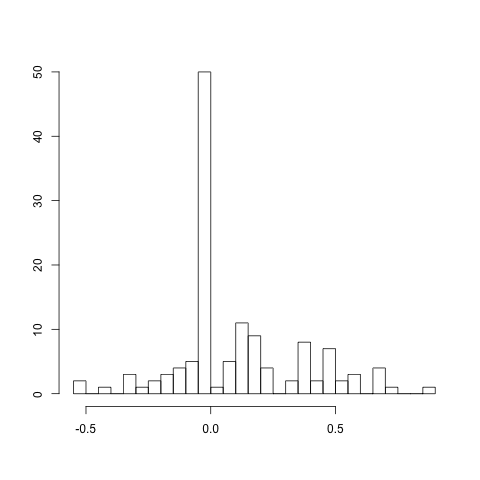
\includegraphics[scale=0.4]{../stats/metricminer-histograma-aspectj.png}
  \caption{The dynamic implementation of the heuristic compared to Emma's in the MetricMiner}
  \label{fig:metricminer-aj}
\end{figure}

\begin{figure}[h!H]
  \centering
  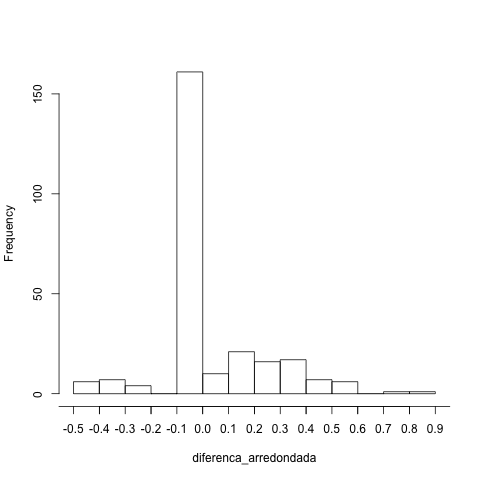
\includegraphics[scale=0.4]{../stats/tubaina-histograma-aspectj.png}
  \caption{The dynamic implementation of the heuristic compared to Emma's in the Tubaina}
  \label{fig:tubaina-aj}
\end{figure}

\begin{figure}[h!H]
  \centering
  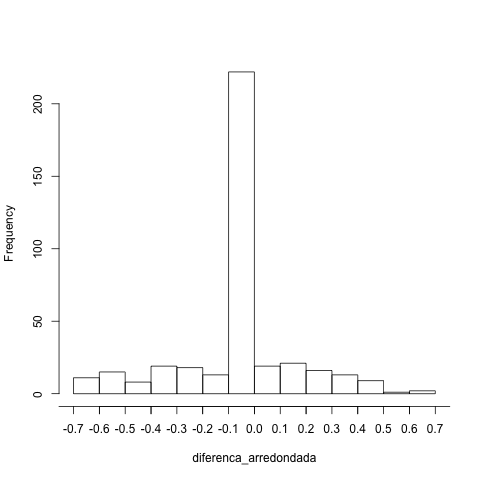
\includegraphics[scale=0.4]{../stats/gnarus-histograma-aspectj.png}
  \caption{The dynamic implementation of the heuristic compared to Emma's in the Gnarus}
  \label{fig:gnarus-aj}
\end{figure}

Based on the numbers we obtained, we believe that the heuristic has an acceptable performance. 
In particular, the maximum mean error found in these 3 projects was 0.1149 (11.5\%). Because of that,
we decided to implement the metric using static analysis. 

%%%%%%%%%%%%%%%%%%%%%%%%%%%%%%%%%%%%%%%%%%%%%%%%%%%%%%%%%%%%%%%%%%%%%%%%%%%%%%%%%%%%%%%%%%
\section{Static Analysis}
\label{sec-results}

As we were satisfied with the results on the proof of concept, we implemented a static tool
to calculate code coverage. It is known that static analysis will never achieve the same performance
found in dynamic analysis: static analysis cannot deal with polymorphism and other concepts from object-orientation.
However, as said before, static analysis is important when dealing with a large set of projects.
The tool we implemented is freely available on Github\footnote{https://github.com/mauricioaniche/gelato2}.

%%TODO: How much exactly is 'most of the data'?
%%TODO: Se Q1 = 0 e Q3 = 0 e se os resultados não estiverem arredondados, isso significa que pelo menos 50 % dos dados são exatamente 0, o que é muito bom
%%TODO: Descrever esses dados com mais rigor
In Figure \ref{fig:metricminer}, we show the histogram of the difference between Emma and our static approach to
the MetricMiner project. By looking to this figure, one can notice that most of the data are between 0 and 0.2. 
The median of the distribution is 0, and the mean is -0.1226. The first quartile is 0, and the
third quartile is also 0.

\begin{figure}[h!H]
  \centering
  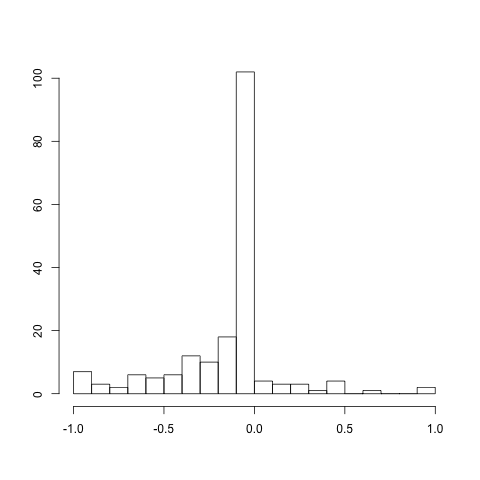
\includegraphics[scale=0.4]{../stats/metricminer-histograma-gelato.png}

  \caption{Our approach compared to Emma's in the MetricMiner}
  \label{fig:metricminer}
\end{figure}

In Figure \ref{fig:tubaina}, from Tubaina project, most of the data are between
0 and -0.2. However, there are also quite a few classes between -1.0 and -0.2. 
The median is -0.1603, and the mean is -0.3074. The first quartile is
-0.6, and the third quartile is 0.

\begin{figure}[h!H]
  \centering
  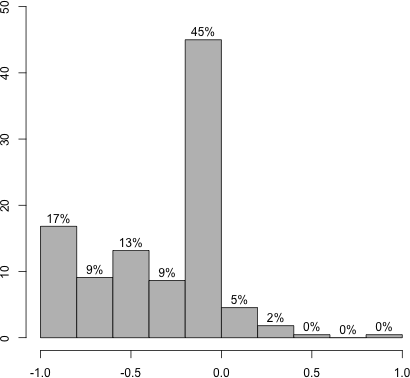
\includegraphics[scale=0.4]{../stats/tubaina-histograma-gelato.png}
  \caption{Our approach compared to Emma's in the Tubaina}
  \label{fig:tubaina}
\end{figure}


In Figure \ref{fig:gnarus}, from Gnarus project, we can see that the data are more varied as 
compared to the previous cases. The median is -0.3852, the mean is -0.3272. The first quartile
is -0.5, and the third quartile is 0.

\begin{figure}[h!H]
  \centering
  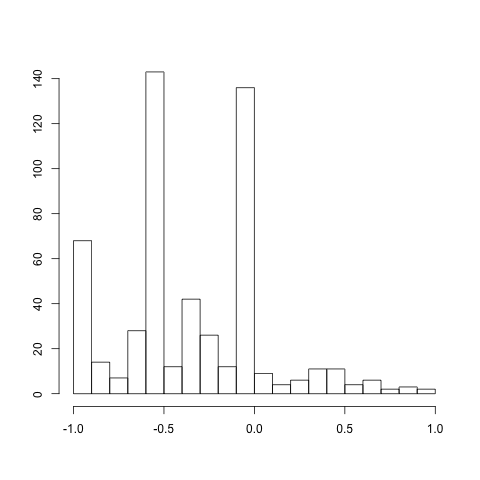
\includegraphics[scale=0.4]{../stats/gnarus-histograma-gelato.png}
  \caption{Our approach compared to Emma's in the Gnarus}
  \label{fig:gnarus}
\end{figure}

By looking to the numbers above, we notice that the implementation was good in the first project,
in which the median was 0, regular in the second one, in which the median was -0.16. However,
in the last project, the heuristic did not go well, as the median was -0.38.

We decided to closely investigate why some classes had such a bad performance. We found out
that our tool was not correctly interpreting a few expressions. In Listing \ref{lst:problem}, we
show an example of a misinterpreted test. In that case, the current implementation of the 
tool does not identify the invocation to \textit{doX()} and \textit{doY()} as both invocations
come from a generic list.

\lstset{caption={The tool does not identify invocations from a list}, label={lst:problem}}
\begin{lstlisting}
List<SomeClass> list = obj.getList();
assertEquals(1, list.get(0).doX());
assertEquals(1, list.get(1).doY());
\end{lstlisting}

Although there were a few implementation problems, we believe that this is a valid approach
when mining repositories.

% TODO: aqui discutir as porcentagens

\section{Threats to Validity}
\label{sec-threats}

There are a few threats to the validity of this research. The first one is that our implementation
still does not fully work: implementing a parser is not an easy task. However, as we showed, the 
heuristic itself seems valid. 

We only evaluated three projects that belong to the same company. It means that these projects
follow basically the same structure, development, and testing rules. That may bias the results.
In a future work, we should run the experiment in many different projects.

%%%%%%%%%%%%%%%%%%%%%%%%%%%%%%%%%%%%%%%%%%%%%%%%%%%%%%%%%%%%%%%%%%%%%%%%%%%%%%%%%%%%%%%%%%
\section{Related Work}
\label{sec-related-work}

Many studies discuss the importance of code coverage when analyzing code quality. 
Sebastian \textit{et al.} \cite{sebastian} say that many software development practices and tools
are based on this number. However, they argue that developers usually calculate it for a single
version of the system, and perform analysis on future versions without recalculating the numbers.
He shows that even relatively small modifications on the source code can affect the code coverage, 
and the impact of the change on the metric is hard to predict.

To the best of our knowledge, there is only one study that discusses the calculation of
code coverage through static analysis. Tiago and Visser \cite{tiago} propose a
technique that uses slicing of static call graphs to estimate the
dynamic test coverage. 
In their approach, they define method coverage as the ratio between covered 
and defined methods per class. They showed that, at system level, the approach
proved to be satisfactory. In package and class level, the difference between
the real and the calculated coverage was small in most cases.

This approach is slightly different from ours. We use McCabe's number to estimate the
minimum number of tests that a class should have. We are also more interested on calculating
code coverage at the class level (from which is possible to derive the system-level number). 
Also, creating a call graph is not simple and takes more effort than just counting
the invoked methods.

%%%%%%%%%%%%%%%%%%%%%%%%%%%%%%%%%%%%%%%%%%%%%%%%%%%%%%%%%%%%%%%%%%%%%%%%%%%%%%%%%%%%%%%%%%
\section{Conclusion and Future Work}
\label{sec-conclusion}

Code coverage is an important metric to analyze software maintenance and evolution. However, it is 
not easy to be calculated, as most tools require compiled code. In this study, we conceived, implemented, 
and evaluated a heuristic to calculate code coverage using static analysis. Apparently, our heuristic can be used 
in mining software repositories studies, as its results were similar to those produced by the popular
code coverage tool Emma. 

As future work, we intend to fix existing bugs in our implementation in order to
achieve better results. Once the desired level of performance is achieved, we intend to implement code coverage
calculation at other levels of abstraction: method, package, and system. Finally, we also 
envision running this same study on more projects from different companies and domains.

% Gustavo: acha que expliquei bem?
In a previous study, we found out that a few developers prefer to write a many different checks in a single
unit test. In our heuristic, even though a method is invoked more than once in a unit test, we count it 
as only one test. A future evaluation would be to consider that the same method can be tested more than once
in a single unit test. That may affect the results, and it needs to be validated.


%%%%%%%%%%%%%%%%%%%%%%%%%%%%%%%%%%%%%%%%%%%%%%%%%%%%%%%%%%%%%%%%%%%%%%%%%%%%%%%%%%%%%%%%%%
\section{Acknowledgments}

We thank \textit{Caelum Ensino e Inovação} for allowing us to run the study in its environment,
as well as supporting the development of the tool.

\bibliographystyle{abbrv}
\bibliography{sigproc}

\end{document}
